\documentclass[conference]{IEEEtran}
\usepackage{graphicx}
\usepackage{multirow}

\usepackage{adjustbox}
\usepackage{algorithm}

\usepackage{algpseudocode}
\usepackage{multirow}

\def\theequation{\arabic{equation}}
\newcommand{\RNum}[1]{\uppercase\expandafter{\romannumeral #1\relax}}
\renewcommand\footnoterule{\hspace{-1em}\rule[0.45em]{\columnwidth}{0.45pt}}
\begin{document}

\title{FedLR: A learning rate based approach towards Efficient communication}

\author{\IEEEauthorblockN{Vipul Singh Negi}
\IEEEauthorblockA{Department of Computer Science and\\Engineering\\National Institute of Technology\\
Rourkela, India 769008\\
vipulhld001@gmail.com}
\and
\IEEEauthorblockN{Suchismita Chinara}
\IEEEauthorblockA{Department of Computer Science and\\Engineering\\National Institute of Technology\\
Rourkela, India 769008\\
suchi.nitrkl@gmail.com}
}



\makeatletter

% \def\ps@IEEEtitlepagestyle{
%   \def\@oddfoot{\mycopyrightnotice}
%   \def\@evenfoot{}
% }
% \def\mycopyrightnotice{
%   {\footnotesize 979-8-3503-0460-2/23/\$31.00~\copyright~2023 IEEE\hfill} % <--- Change here
%   \gdef\mycopyrightnotice{}
% }



% \IEEEoverridecommandlockouts
% \IEEEpubid{\makebox[\columnwidth]{979-8-3503-0460-2/23/23/\$31.00~\copyright2023 IEEE \hfill} \hspace{\columnsep}\makebox[\columnwidth]{ }}

% \makeatletter

% \def\ps@IEEEtitlepagestyle{
%   %\def\@oddfoot{\mycopyrightnotice}
%   \def\@evenfoot{}
% }
% \makeatletter
% \def\footnoterule{\kern-3\p@
%   \hrule \@width 2in \kern 2.6\p@} % the \hrule is .4pt high
% \makeatother
% \newcommand{\copyrightnotice}[1]{{%
%   \renewcommand{\thefootnote}{}% Remove footnote number
%   \footnotetext[0]{#1}%
% }}
\maketitle
% \copyrightnotice{979-8-3503-0460-2/23/\$31.00~\copyright~2023 IEEE}
% \IEEEpubidadjcol

\begin{abstract}
The challenges of handling decentralised data lead to the demand for research on secure gathering, efficient processing, and analysing of the data. In decentralised systems, each node (device) can make independent decisions, reducing the complexity and challenges of dealing with extensive data. Privacy has become a significant concern for our society due to the rise in the number of Edge/IoT devices, the lack of presence of a centralised system, etc. To solve this conundrum, federated learning was proposed. Federated learning works on the sharing of parameter values rather than the data. Worldwide, 10.2 Billion non-IoT and 19.8 billion IoT devices will be active in 2023. These devices lack security when it comes to using traditional machine learning. However, federated learning models solve this problem using techniques such as Secure Aggregation and Differential Privacy, which provide security for the devices and efficient communication between them. The challenges arise from heterogeneous devices, leading to the client selection problem, unbalanced data, and many more problems. The Proposed work focuses on using the MobileNets series of model architecture for federated learning using the FedAvg Strategy. MobileNets architecture has always been robust and reliable when it come to devices with resource constraints. An older generation system is used to show that federated learning is a viable technique for decentralized machine learning.
\end{abstract}
\begin{IEEEkeywords}
Federated learning, IoT, Deep Learning, MobileNets
\end{IEEEkeywords}

\IEEEpeerreviewmaketitle



\section{Introduction}
Federated Learning is born at the intersection of Edge computing/IoT, on-device AI, and blockchain.  A Federation refers to a group of independent entities yet united under a central organization. In federated learning, multiple client or organisations share their training data (weights or compute) to remote servers, and all the clients participating in the process train a single neural network. This process is repeated by the clients, downloading the newer weights from the servers multiple times to provide better results. The training is done on the device's private data, then it is encrypted and communicated to the server, and on the server, they are decrypted, averaged, and integrated into
the centralized model. The main objective of federated learning is to converge the client's weights so that it could yield meaningful results. For Example. WeBank (Banking), NVIDIA Clara
(Healthcare), and Google Keyboard.\par
WeBank is a private Chinese bank they have created its own federated learning framework, known as WeBankAI (based on FATE) \cite{liu2021fate}. Nvidia Clara \cite{nvidia} is a platform to improve healthcare that focuses on \cite{liu2021fate} Medical Imaging and Medical Devices (Nvidia Clara Holoscan), Healthcare IoT (Nvidia Clara Guardian Collection), Biopharma (BioNeMo), and Genomics (Nividia Clara Parabricks). Google Keyboard (Gboard) \cite{yang2018applied} has been using federated learning for creating word prediction models.\par
Google introduced the term federated learning in 2016 (coined in 2017 by McMahan et al. \cite{mcmahan2017communication}), about the same time the Cambridge Analytica scandal awakened users of the dangers of sharing personal information online. It started a revolution in the technology world about the three rules of Cryptography confidentiality, integrity, and availability. After a deeper review of our current laws, it was clear that we had none. So laws like GDPR and CCPA came into regulation. Federated Learning (Fig \ref{fig1}.) is one such method which can satisfy the rules of cryptography and privacy laws around the globe.\par 

\begin{figure}[htp!]
	\centering
	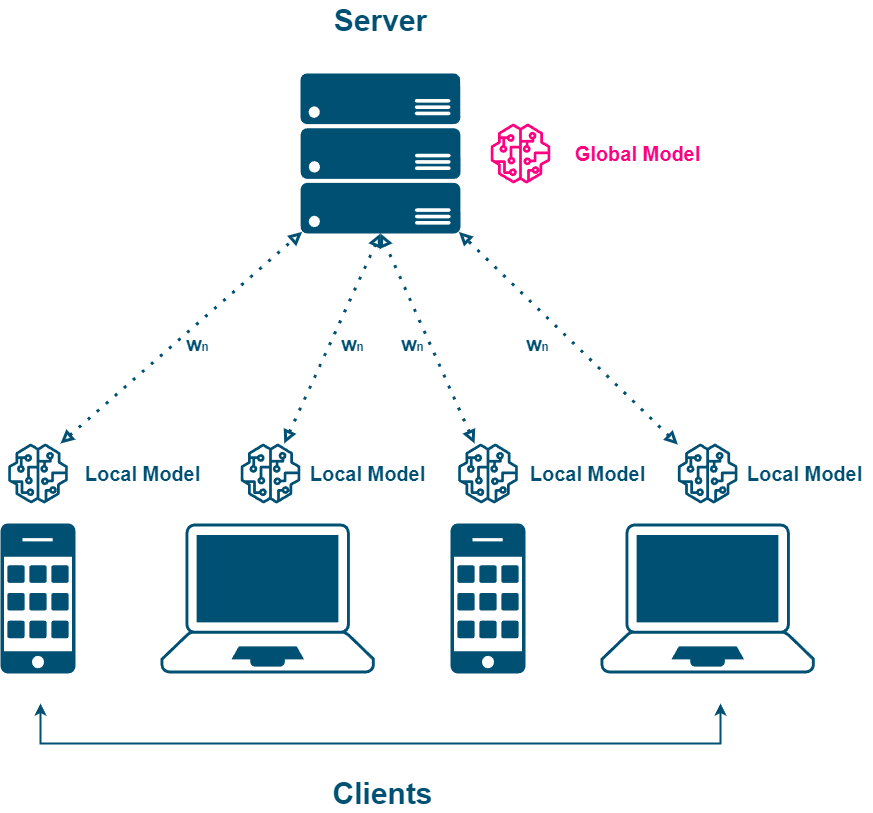
\includegraphics[scale=.25]{Images/FEDLEARN_NEW}
	\caption{Workings of Federated Learning.}
	\label{fig1}
\end{figure}

 In this paper we present a new strategy which significantly addresses the problem with the old one keeping the effectiveness of federated learning alive. The main problem with the vanilla FedAvg is the client selection methodology which is taken at random and the devices participation have no threshold value to meet in order to participate in the federated learning process. Another problem with FedAvg is to deal with device heterogeneity as each devices usually tend to have different CPU, RAM, and GPU which are the essential blocks of any neural network. FedProx \cite{li2020federated} remedies the heterogeneity of FedAvg to a certain point but doesn't account for the fairness. Fairness means all clients should be treated as fair and their contributions to the global model should carry equal weight. The proposed strategy has been named as FedLR which is a dynamic learning rate and epoch based client  selection 3strategy.
 
 The proposed work focuses on reducing the total communication time taken by federated learning. Chen et al. \cite{chen2023boosting} used RAM and CPU utilization data from clients in order to boost client selection. But getting such data from clients could lead to device fingerprinting \cite{radhakrishnan2014gtid} \cite{patwari2022dnn} which puts federated learning at risk.  In this paper, by considering heterogeneous clients, we are employing FedLR, a learning rate based towards efficient communication. In the proposed methodology a time variable has been calculated and according to that time variable qualitative decisions towards learning rate selection has been made.
FedLR guarantee faster communication time with fair selection of clients as it always consider slacker devices which makes this methodology Fair. The main contribution of the proposed work are summarized as follows:
\begin{enumerate}
	\item By conducting extensive sets of experiments we came to a quantitative conclusion about the effects of learning rate (lr) in federated learning which is highly effective parameter in federated learning.
	\item The next contribution is regarding individual clients epochs. The time variable which represents each clients runtime is used to find out the slacker devices and adjust the epoch values for reducing the number of slacker devices.
	\item Pairing the time variable with lr and epoch values of client to perform better client selection which focused on fairness and heterogeneity. A client selection strategy FedLR has been proposed.
\end{enumerate}

The ultimate goal of this work is to present a federated learning approach which reduces the communication cost as well as preserves the Accuracies of the clients model. The remainder of the paper is organized as follows: Section \RNum{2} discusses Related Works. Section \RNum{3} explains the problem statement of the literature. Section \RNum{4} introduces FedLR and explains its key features and how does it perform them. Section \RNum{5} does result and analysis of the proposed algorithm and Section \RNum{6} finally concluding this paper.


\section{Related Works}
The idea of privacy-preserving deep learning was first presented by Shokri et al. \cite{shokri2015privacy} using distributed and selective SGD to make deep learning models privacy-preserving. After this the Federated learning terminology was coined by McMahan et al. \cite{mcmahan2017communication} in which they proposed the Federate Averaging algorithm and tested it using the MNIST Digit Dataset. The data was partitioned into IID and Non-IID. In Non-IID data, only two-digit data were given to the clients. They have also used CIFAR-10 in the balanced and IID settings. 
 \par
Khan et al. \cite{khan2021federated} and Nguyen et al. \cite{nguyen2021federated} have talked about advancements in federated learning for IoT, taxonomy and the open challenges. A state-of-the-art survey on the use of Federated Learning in smart healthcare. Advances in Federated Learning design for healthcare addressing resource-aware federated learning, security and privacy federated learning. \par
Nishio et al. \cite{nishio2019client} proposed a new strategy for client selection in federated learning. The strategy is coined as FedCS (Federated Learning with Client Selection). They have added an extra step in the original FedAvg called Resource Request which gathers the client's resource information and groups them according to their resource capacity. They have also used schedule updates and upload and compared their results in both IID and Non-IID datasets.
\par
Abdulrahaman et al. \cite{abdulrahman2020fedmccs} proposed a multicriteria-based client selection (The server analyzes the client's responses to select the best set able to participate in the coming learning rounds). They have also added client filtering similar to \cite{nishio2019client}. They are not choosing clients at random rather; they are using Stratified Sampling.
\par
Saha et al. \cite{saha2020fogfl} proposed fog-assisted federated learning for resource-constrained IoT devices. They have created a fog fl framework and formulated a greedy heuristic strategy to select the optimal global aggregator fog nodes at the end of an epoch to increase the reliability of the system. They have compared their findings with FedAvg and HFL. Mathur et al. \cite{mathur2021device} has implemented federated learning using the Flower framework. They have implemented federated learning in 5 mobile devices (three phones and two tablets). They used CIFAR-10 and Office-31 datasets in their experiments. They have evaluated their finding in terms of the local epoch, accuracy, convergence time (mins), and energy consumed by (kJ) the device. They have used the ever-popular MobileNetV2 \cite{sandler2018mobilenetv2} architecture. 
\par Li et al. \cite{li2020federated} proposed an update to the traditional FedAvg by adding statistical heterogeneity (Proxmial Term) which handles clients heterogeneity better than the previously proposed method.  \par Wang et al. \cite{wang2023applications} have talked about Statistical heterogeneity, communication cost, system heterogeneity, real-time etc, in the mHealth setting showing Federated Learning is also suitable for mobile health applications. Providing a real time benefit of privacy preserving Deep Learning. 

\section{Problem Statement}
The FedAvg proposed by \cite{mcmahan2017communication} open the doors for communication-efficient deep learning networks as they proposed the Federated Averaging methods to train models collaboratively without sharing the underlying training data to preserve the privacy and ever since then it have become the state of the art method for Privacy preserving Deep Learning Models. 
\subsection{Problem Setup} 
The vanilla FedAvg algorithm has some problems when it comes to client selection, heterogeneous computational resources, and fairness. As it focuses primarily on the privacy preserving aspect of the learning. The algorithm begins with initializing the global model at random or for pre-trained data. The beings the client selection process which selects clients at random. The global weights are distributed to the clients and the training begins and only stops when we get our desired outcome. To remedy the heterogeneity of FedAvg a new stategy FedProx \cite{li2020federated} was proposed which try to contain the dropping slacker devices due to the heterogeneous nature of the devices.

\subsection{Client Selection}

In the vanilla FedAvg the clients are selected at random using 
\begin{equation}
 m \gets max(C\cdot K,1)
 \label{eq1}
 \end{equation}
 where C is the fraction of selected clients and K being the actual clients which gives us the total number of m clients for the federated learning. This method of selection client is good but it can easily be improved upon by proposing a new strategy for client selection by adding some more criteria for client selection. The proposed strategy should improve over the existing one by making the process more robust and highly communication efficient. A new parameter is required which can perform better client selection the current Equation \ref{eq1}.   

\subsection{Heterogeneous Computational Resources}
The devices participating in the federated learning are not always homogeneous the chances of it being heterogeneous are more. A survey done by Markets and Markets \cite{market} states that 35 key players exist in the edge devices manufacturing phase with some providing devices while other provides the processors. This many key players means that major amount of devices are heterogeneous which makes client selection much more complicated because as the diversity increases the number of slacker devices also increases. Slacker devices are the devices which are slowest performer in the system. The motto of federated learning is the faster the slacker device the model will be equally efficient. So that means in order to propose a better strategy one must figure out a way to improve upon the slacker devices. 

\subsection{Fairness}
Fairness is an unique thing which removes the discrimination between clients and making sure all the devices contribution are taken into consideration. The best way to understand this problem is to imagine two hospitals H1 and H2 with H1 being a bigger hospital with various specialization and H2 being a small clinic. Communicable Diseases are the most popular ones and easy to get and if H1 is getting patient for one such communicable disease that means is the same for H2 are well. But due to the size of H1 the data gathered from H2 will be minuscule but that doesn't mean that its irrelevant. So one must also consider fairness as one of the major components for creating a new strategy. Ezzeldin et al. \cite{ezzeldin2023fairfed} has proposed a Fairfed strategy to solve this problem using debiasing method across clients.
 
\section{Proposed Algorithm: FedLR}
The proposed FedLR is broken into three segments: Learning Rate Selection, Epoch Selection for individual clients, and Client Selection based on the Client Runtime. The objective it to reduce the communication cost for efficient communication all the while preserving the accuracy of the model. A slacker device-centric algorithm has been proposed, focusing on the slowest devices and considering the fairness of client selection. A Federated Learning System is as fast as its slowest device. This is the basic principle of federated learning, so the proposed algorithm for client selection primarily focuses on optimizing the slowest devices in the federation. The algorithm is based on turning the learning rate and epochs of Individual clients. A time quantum has been proposed; the clients are classified as quicker or slacker based on the help of this time quantum. To validate if the learning rate based assumption (Section IV A) is correct (the bigger and smaller lr are assigned for quicker and slacker devices, respectively). However, this will only reduce the total communication time by a few seconds, so a new epoch for the slacker devices is proposed below in equation \ref{epoch_equation}. to make it effective (Section IV B).
 \subsection{Learning Rate Selection}
The algorithm \ref{alg:lr} below explains the learning rate (lr) selection by the clients. The learning rates are taken with an increment of ten. After running different lr it was observed that the accuracy were similar but the total communication times were being reduced with smaller lr values. All three lr cases were tested and they showed a good amount of change in communication cost. The dataset used for these experiments was the CIFAR10 dataset.

 
 \begin{algorithm}
 	\scriptsize
 	\caption{ \textbf{Learning Rate Selection} The $K$ clients are
 		indexed by $k$; $B$ is the local minibatch size, $E$ is the number
 		of local epochs, and $\eta$ is the learning rate}\label{alg:lr}
 	\begin{algorithmic}[1]
 		
 		
 		\State \textbf{ClientUpdate($k,W$):} \Comment{Run on client $k$}
 		\State $\mathcal{B} \gets$ (split $\mathcal{P}_k$ into batches of size $B$)
 		\For{\texttt{each local epoch $i$ from 1 to $E$ }}
 		\State Fit $\eta$ as [0.01, 0.001, 0.0001] from the Server.
 		\For{\texttt{batch $b \in \mathcal{B}$ }}
 		\State $w \gets w - \eta \nabla l(w;b)$
 		\EndFor
 		\EndFor
 		\State return $w$ to server
 		
 	\end{algorithmic}
 \end{algorithm}
 
 \subsubsection{Case 1: FedLr (lr =0.01) with 10 Rounds and 5 Epochs}
 
 The best accuracy we achieved in this scenario is 56.6\%. This works similarly to the FedAvg Strategy and claims almost similar runtime the gap is 2s. The losses also perform similarly to the base FedAvg Strategy. Table \ref{lrsmall} shows the result of the experiment.
 \begin{table}[ht]
 	\centering
 	\caption{FedLr (lr =0.01) with 10 Rounds and 5 Epochs}
 	\resizebox{\columnwidth}{!}{%
 		\begin{tabular}{|lllllc|}
 			\hline
 			\multicolumn{6}{|c|}{FedLR (lr = 0.01) with 10 Round and 5 Epochs}                                                                                                                                     \\ \hline
 			\multicolumn{1}{|l|}{Clients} & \multicolumn{1}{l|}{Accuracy}        & \multicolumn{1}{l|}{Loss}  & \multicolumn{1}{l|}{Local Acc} & \multicolumn{1}{l|}{Local Loss} & \multicolumn{1}{l|}{Total Time} \\ \hline
 			\multicolumn{1}{|l|}{1}       & \multicolumn{1}{l|}{56.2\%}          & \multicolumn{1}{l|}{0.063} & \multicolumn{1}{l|}{95.3\%}    & \multicolumn{1}{l|}{0.0050}     & \multirow{5}{*}{835.6s}         \\ \cline{1-5}
 			\multicolumn{1}{|l|}{2}       & \multicolumn{1}{l|}{52.4\%}          & \multicolumn{1}{l|}{0.065} & \multicolumn{1}{l|}{95.7\%}    & \multicolumn{1}{l|}{0.0047}     &                                 \\ \cline{1-5}
 			\multicolumn{1}{|l|}{3}       & \multicolumn{1}{l|}{51.2\%}          & \multicolumn{1}{l|}{0.069} & \multicolumn{1}{l|}{94.7\%}    & \multicolumn{1}{l|}{0.0053}     &                                 \\ \cline{1-5}
 			\multicolumn{1}{|l|}{4}       & \multicolumn{1}{l|}{\textbf{56.6\%}} & \multicolumn{1}{l|}{0.068} & \multicolumn{1}{l|}{94.6\%}    & \multicolumn{1}{l|}{0.0056}     &                                 \\ \cline{1-5}
 			\multicolumn{1}{|l|}{5}       & \multicolumn{1}{l|}{52.4\%}          & \multicolumn{1}{l|}{0.061} & \multicolumn{1}{l|}{94.9\%}    & \multicolumn{1}{l|}{0.0054}     &                                 \\ \hline
 		\end{tabular}%
 		}\label{lrsmall}
 \end{table}   
 
 %%%%%%%%%%%%%%%%%%%%%%%%%%%%%%%%%%%%%%%%%%%%%%%%%%%%%%%%%%%
 \subsubsection{Case 2: FedLr (lr =0.001) with 10 Rounds and 5 Epochs}
 % Please add the following required packages to your document preamble:
 % \usepackage{multirow}
 % \usepackage{graphicx}
 The best accuracy is 56.2\%. The runtime is reduced by 6 seconds, which makes it half a second per round. However, the losses are greater compared to Case 1. In Case 1, the lowest loss was 0.0047; in Case 2, it was 0.0066. Table \ref{lrmid} shows the result of this experiment.
 \begin{table}[ht]
 	\centering
 	\caption{FedLr (lr =0.001) with 10 Rounds and 5 Epochs}
 	%\resizebox{\columnwidth}{!}{%
 		\begin{tabular}{|lllllc|}
 			\hline
 			\multicolumn{6}{|c|}{FedLR (lr = 0.001) with 10 Round and 5 Epochs}                                                                                                                             \\ \hline
 			\multicolumn{1}{|l|}{Clients} & \multicolumn{1}{l|}{Accuracy} & \multicolumn{1}{l|}{Loss}  & \multicolumn{1}{l|}{Local Acc} & \multicolumn{1}{l|}{Local Loss} & \multicolumn{1}{l|}{Total Time} \\ \hline
 			\multicolumn{1}{|l|}{1}       & \multicolumn{1}{l|}{55.8\%}   & \multicolumn{1}{l|}{0.065} & \multicolumn{1}{l|}{93.4\%}    & \multicolumn{1}{l|}{0.0066}     & \multirow{5}{*}{830.9s}         \\ \cline{1-5}
 			\multicolumn{1}{|l|}{2}       & \multicolumn{1}{l|}{56\%}     & \multicolumn{1}{l|}{0.059} & \multicolumn{1}{l|}{93.7\%}    & \multicolumn{1}{l|}{0.0064}     &                                 \\ \cline{1-5}
 			\multicolumn{1}{|l|}{3}       & \multicolumn{1}{l|}{52.4\%}   & \multicolumn{1}{l|}{0.069} & \multicolumn{1}{l|}{93.5\%}    & \multicolumn{1}{l|}{0.0067}     &                                 \\ \cline{1-5}
 			\multicolumn{1}{|l|}{4}       & \multicolumn{1}{l|}{52.4\%}   & \multicolumn{1}{l|}{0.069} & \multicolumn{1}{l|}{93.7\%}    & \multicolumn{1}{l|}{0.0065}     &                                 \\ \cline{1-5}
 			\multicolumn{1}{|l|}{5}       & \multicolumn{1}{l|}{\textbf{56.2\%}}   & \multicolumn{1}{l|}{0.059} & \multicolumn{1}{l|}{93.4\%}    & \multicolumn{1}{l|}{0.0066}     &                                 \\ \hline
 		\end{tabular}%
 		%}
 		\label{lrmid}
 \end{table}
 
 %%%%%%%%%%%%%%%%%%%%%%%%%%%%%%%%%%%%%%%%%%%%%%%%%%%%%%%%%%%
 \subsubsection{Case 3: FedLr (lr =0.0001) with 10 Rounds and 5 Epochs}
The best accuracy is 57.6\% with runtime reduced by 9 sec. While having similar losses as Case 1 and 2. The full results are in table \ref{lrlarge} below.
 \begin{table}[ht]
 	\centering
 	\caption{Case 3 : FedLr (lr =0.0001) with 10 Rounds and 5 Epochs}
 	%\resizebox{\columnwidth}{!}{%
 		\begin{tabular}{|lllllc|}
 			\hline
 			\multicolumn{6}{|c|}{FedLR (lr = 0.0001) with 10 Round and 5 Epochs}                                                                                                                            \\ \hline
 			\multicolumn{1}{|l|}{Clients} & \multicolumn{1}{l|}{Accuracy} & \multicolumn{1}{l|}{Loss}  & \multicolumn{1}{l|}{Local Acc} & \multicolumn{1}{l|}{Local Loss} & \multicolumn{1}{l|}{Total Time} \\ \hline
 			\multicolumn{1}{|l|}{1}       & \multicolumn{1}{l|}{54.8\%}   & \multicolumn{1}{l|}{0.063} & \multicolumn{1}{l|}{93\%}      & \multicolumn{1}{l|}{0.0060}     & \multirow{5}{*}{826.0s}         \\ \cline{1-5}
 			\multicolumn{1}{|l|}{2}       & \multicolumn{1}{l|}{\textbf{57.6\%}}   & \multicolumn{1}{l|}{0.062} & \multicolumn{1}{l|}{95\%}      & \multicolumn{1}{l|}{0.0053}     &                                 \\ \cline{1-5}
 			\multicolumn{1}{|l|}{3}       & \multicolumn{1}{l|}{56.8\%}   & \multicolumn{1}{l|}{0.063} & \multicolumn{1}{l|}{95.2\%}    & \multicolumn{1}{l|}{0.0050}     &                                 \\ \cline{1-5}
 			\multicolumn{1}{|l|}{4}       & \multicolumn{1}{l|}{54.4\%}   & \multicolumn{1}{l|}{0.065} & \multicolumn{1}{l|}{95.1\%}    & \multicolumn{1}{l|}{0.0052}     &                                 \\ \cline{1-5}
 			\multicolumn{1}{|l|}{5}       & \multicolumn{1}{l|}{53.4\%}   & \multicolumn{1}{l|}{0.062} & \multicolumn{1}{l|}{94.6\%}    & \multicolumn{1}{l|}{0.0056}     &                                 \\ \hline
 		\end{tabular}%
 		%}
 		\label{lrlarge}
 \end{table}

\subsection{Epoch Selection for Individual Clients}
The first step was to figure out suitable lr values which provides us with significant changes but just changing the lr values in not sufficient for us to make the strategy robust. The next step is to provide individual epoch values for each client based on a balanced parameter. Chen et al. \cite{chen2023boosting} used CPU and RAM metric of clients in order to boost their strategy. This methodology is effective but is not fully privacy preserving. Device fingerprinting is a big risk to the Federated Learning scenario.  Li et al. \cite{li2020federated} proposed a Proximal term to improve the slacker devices which were dropping because of delays in computing $E$. The proposed equation \ref{epoch_equation} calculate local epochs for individual clients.

\begin{equation}
	E_n = \left \lfloor\frac{mode[T_q] - count\_of\_value}{mode[T_q]}\right \rfloor * E 
	\label{epoch_equation}
\end{equation}
In Equation \ref{epoch_equation}.\textit{ $mode[T_q]$} is the mode value from the time quantum, and \textit{count\_of\_value} is the time the mode value is repeated. The equation \ref{epoch_equation} combined with the equation \ref{eq1} for client selection improves it significantly.
The key values for the Algorithm \ref{alg:cap} are as follows:
\begin{enumerate}
	\item The K clients are indexed by k.
	\item C is the fraction of the client selected.
	\item B is the local minibatch size.
	\item E is the number of local epochs.
	\item $\eta$ is the learning rate.
	\item $T_q$ is time quantum.
	\item $E_n$ is the new epoch.
\end{enumerate}

\begin{algorithm}[H]
	\scriptsize
	\caption{ \textbf{FedLR} The $K$ clients are
		indexed by $k$; $B$ is the local minibatch size, $E$ is the number
		of local epochs and $E_n$ is the new epoch, $T_q$ is the time quantum, and $\eta$ is the learning rate}\label{alg:cap}
	\begin{algorithmic}[1]
		
		\State \textbf{Server Executes}
		\State initialize $w_0$
		\For{\texttt{each round $t$ = 1,2,..}}
		\State \texttt{$m \gets max(C\cdot K,1)$}
		\State \texttt{$S_t \gets $(random set of $m$ clients)}
		\For{\texttt{each client $k \in S_t $ }\textbf{in parallel}}
		\State $w_{t+1}^{k} \gets ClientUpdate(k,w_t)$
		\EndFor
		\State $w_{t+1} \gets \sum_{k=1}^{K} \frac{n_k}{n} w_{t+1}^{k}$
		
		\EndFor
		\State \textbf{ClientUpdate($k,W$):} \Comment{Run on client $k$}
		\State $\mathcal{B} \gets$ (split $\mathcal{P}_k$ into batches of size $B$)
		\For{\texttt{each local epoch $i$ from 1 to $E$ | $E_n$ }}
		\State Find $T_q$ ($T_q$ is the epoch runtime of individual clients).
		\State Find mode[$t_q$]
		\State \textbf{if:} mode[$t_q$] is smallest 
		\State \hspace{.3cm} i = E and $\eta$= Bigger Learning Rate
		\State \textbf{else:} 
		\State \hspace{.3cm} Find $E_n$ using equation 1. 
		\State \hspace{.3cm} i = $E_n$ and $\eta$ = Smaller Learning Rate
		\For{\texttt{batch $b \in \mathcal{B}$ }}
		\State $w \gets w - \eta \nabla l(w;b)$
		\EndFor
		\EndFor
		\State return $w$ to server
		
	\end{algorithmic}
\end{algorithm}
 

\subsection{Working of FedLR}
\begin{figure}[htp!]
	\centering
	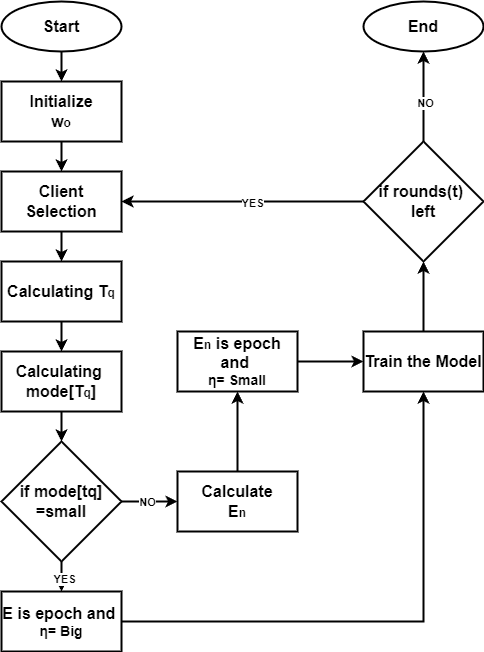
\includegraphics[scale=.28]{Images/Result Images/Flow_FedLR }
	\caption{Flow Chart describing the workings of FedFL.}
	\label{FlowFedLR}
\end{figure}
Fig. \ref{FlowFedLR} shows the workings of FedLR. Initialize the global parameter value $w_0$.Selection of all the eligible clients for training.Finding each client’s run-time as they finish training. Finding the mode time value by comparing the individual times. Selecting the learning rate and epoch values based on the mode value. The bigger learning rate ($\eta$) will be assigned to quicker devices with the default epoch ($E$) value. The slacker devices will be assigned a lower learning rate with a lower epoch value En using equation \ref{eq1}. and a smaller $\eta$. The time of these devices will be compared next, and the
slacker devices will receive a low amount of work but will still be a pivotal element in the federated learning process.

\section{Result and Analysis}
The model architecture used in the experiments is a 2 layered Convolution Neural Network. The list of datasets used for the experiments are as follows:
\begin{enumerate}
    \item CIFAR10 \cite{cifar10} dataset containing ten classes.
    \item MNIST \cite{lecun1998mnist} dataset of Handwritten digits containing ten classes. 
    \item FMNIST \cite{xiao2017fashionmnistnovelimagedataset} dataset of fashion items containing ten classes.
    \item CIFAR100 \cite{Krizhevsky09learningmultiple} dataset containing hundred classes. 
\end{enumerate}
\subsection{Machines Used}
Two machines are used to test the proposed algorithm, and the specifications of the machines are given below:
\begin{enumerate}
	\item Google Collab (Free Tier with T4 GPU).
	\item Workstation (128GB RAM, Intel Xeon Silver 4216 CPU, and NVIDIA RTX A4000 GPU)
\end{enumerate}

All clients use the full datasets and run at 10 Epochs and 10 Communication Rounds. Using .25 and 1 GPU and CPU, respectively in Flower. The Results of our Experiments are as follows:
10 Clients using FedAvg, FedProx, and FedLR on the all Datasets. The blue dotted lines represents the local loss and accuracy while the orange ones represent the global loss and accuracy. The legends shows how many total epochs does one client take.

\begin{figure}[htp!]
	\centering
	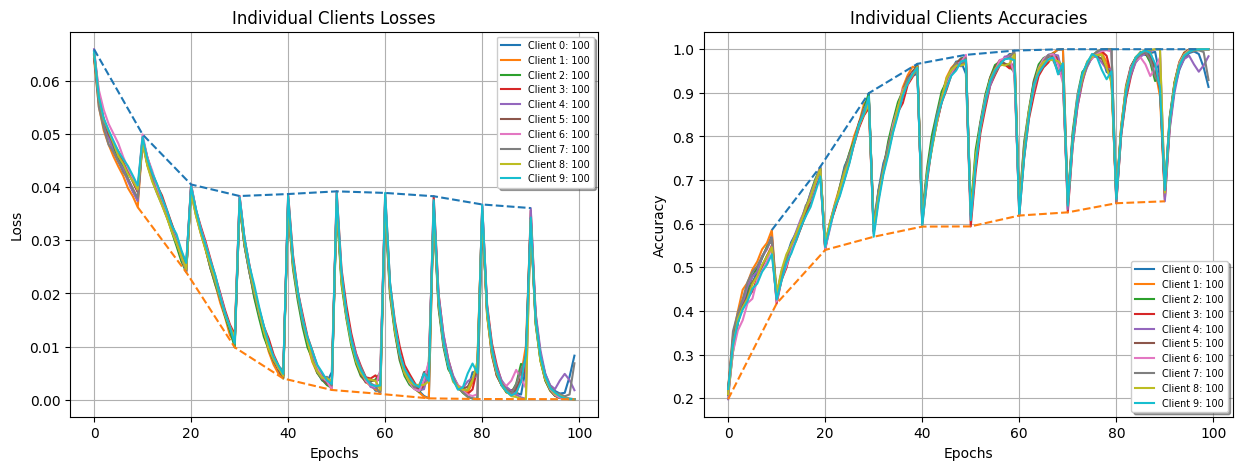
\includegraphics[scale=.28]{Images/Result Images/CIFAR 10/cifar10_fedavg_lossacc }
	\caption{Accuracy and Loss of 10 Clients using FedAvg on the CIFAR10 Dataset (Workstation).}
	\label{FedAvgC10}
\end{figure}

\begin{figure}[htp!]
	\centering
	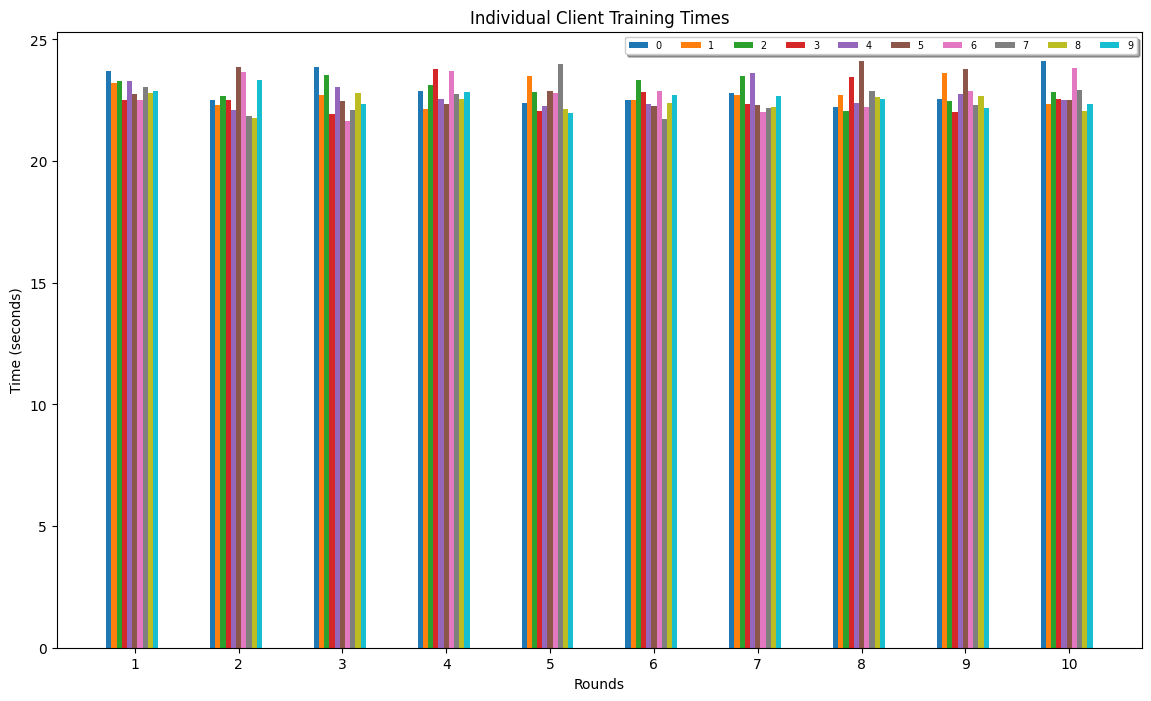
\includegraphics[scale=.3]{Images/Result Images/CIFAR 10/cifar10_fedavg_total_time_635o65 }
	\caption{Individual Time of 10 Clients using FedAvg on the CIFAR10 Dataset (Workstation).}
	\label{FedAvgTimeC10}
\end{figure}

Fig. \ref{FedAvgC10} and \ref{FedAvgTimeC10} represents the accuracy loss plot and Individual time taken by each client respectively for FedAvg.  These are workstation times and the accuracy and losses are similar to FedLR and FedProx. The blue dotted lines represents the local loss and accuracy while the orange ones represent the global loss and accuracy. The legend of the fig. \ref{FedAvgC10} shows how many total epochs does one client take.

Fig. \ref{FedProxC10} and \ref{FedProxTimeC10}  represents the accuracy loss plot and Individual time taken by each client respectively for FedProx. FedProx perform a bit better in terms of total communication cost.
\begin{figure}[htp!]
	\centering
	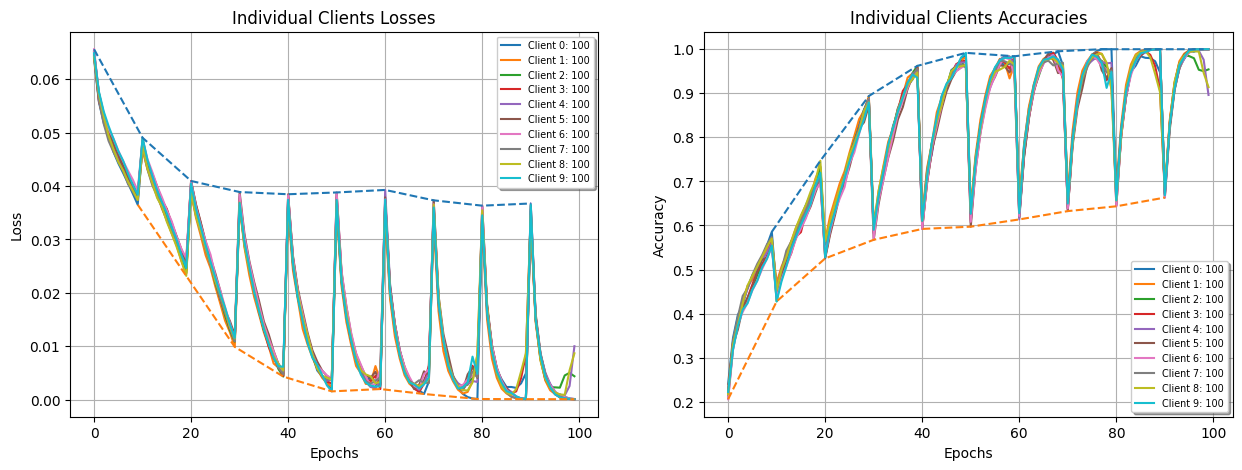
\includegraphics[scale=.28]{Images/Result Images/CIFAR 10/cifar10_fedPROX_lossacc }
	\caption{Accuracy and Loss of 10 Clients using FedProx on the CIFAR10 Dataset (Workstation).}
	\label{FedProxC10}
\end{figure}

\begin{figure}[htp!]
	\centering
	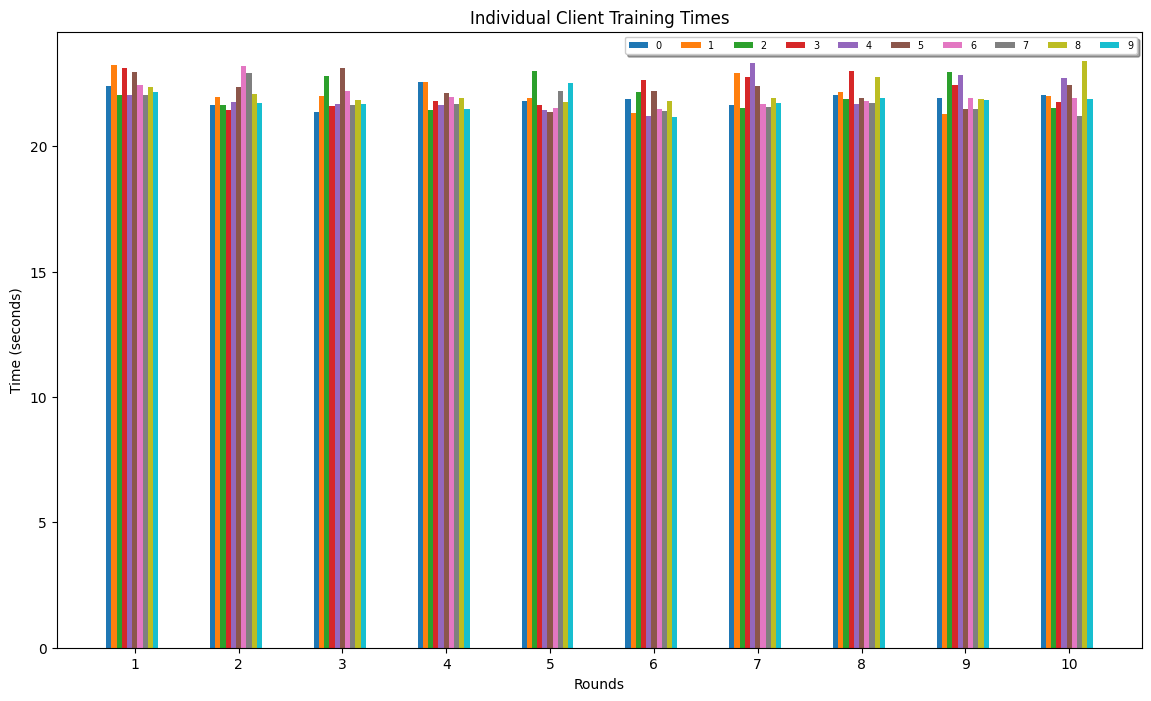
\includegraphics[scale=.3]{Images/Result Images/CIFAR 10/cifar10_fedPROX_total_time_622o28 }
	\caption{Individual Time of 10 Clients using FedProx on the CIFAR10 Dataset (Workstation).}
	\label{FedProxTimeC10}
\end{figure}



\begin{figure}[htp!]
	\centering
	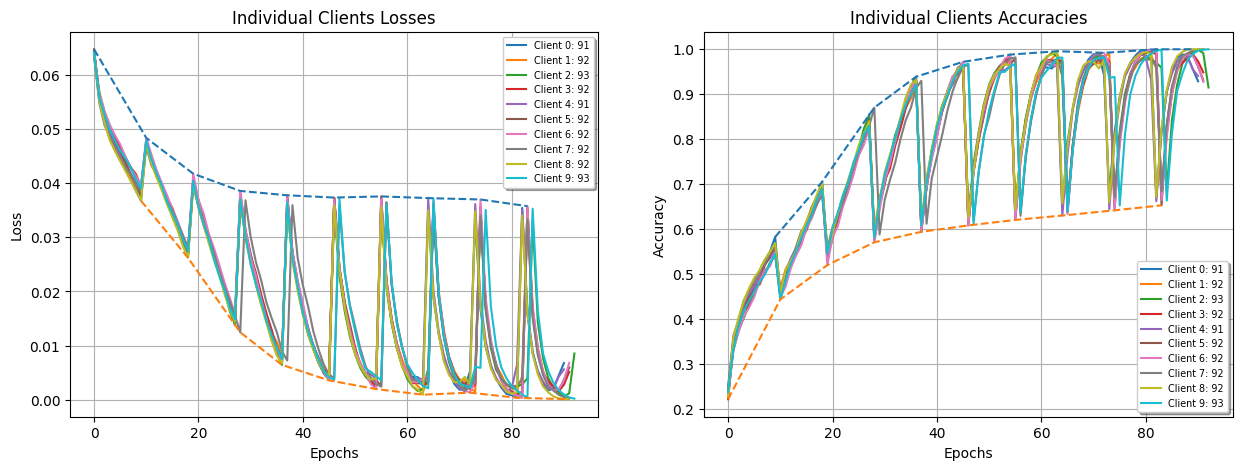
\includegraphics[scale=.28]{Images/Result Images/CIFAR 10/cifar10_mystrat_lossacc }
	\caption{Accuracy and Loss of 10 Clients using FedLR on the CIFAR10 Dataset (Workstation).}
	\label{FedLRC10}
\end{figure}

\begin{figure}[htp!]
	\centering
	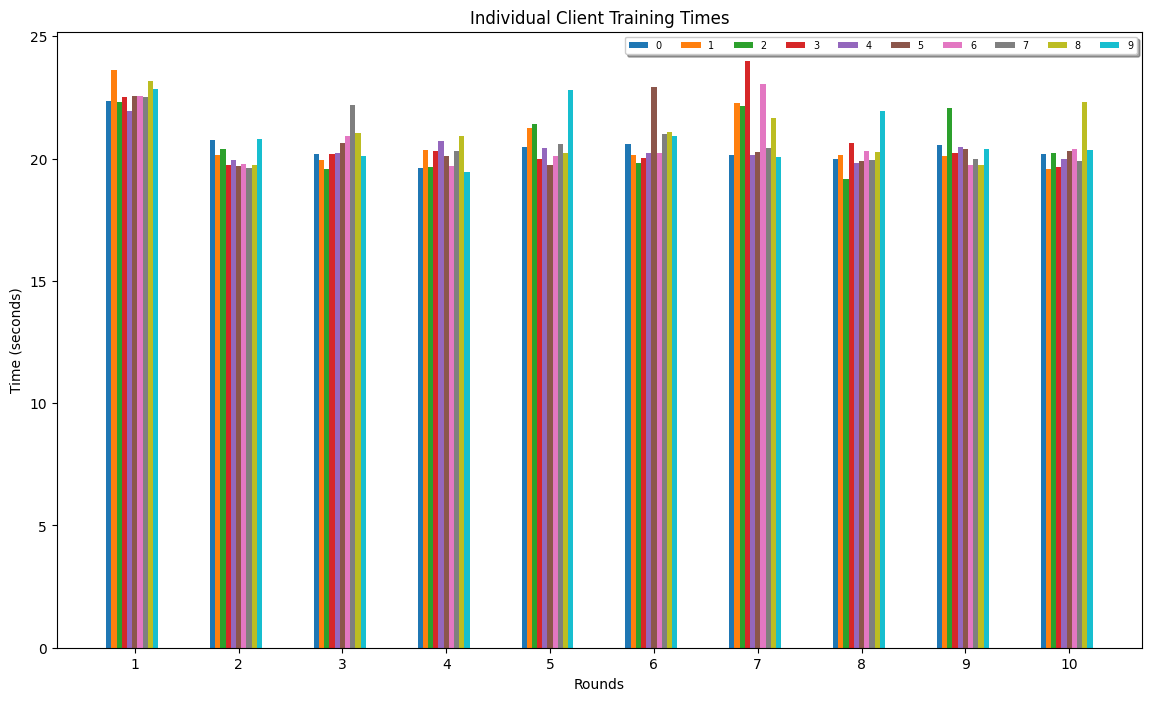
\includegraphics[scale=.3]{Images/Result Images/CIFAR 10/cifar10_total_time_589o74 }
	\caption{Individual Time of 10 Clients using FedLR on the CIFAR10 Dataset (Workstation).}
	\label{FedLRTimeC10}
\end{figure}
Fig. \ref{FedLRC10} and \ref{FedLRTimeC10} represents the accuracy loss plot and Individual time taken by each client respectively for FedLR. In fig. \ref{FedLRC10} each client runs a different number of epoch. The one with the lowest epochs are the Slacker devices hence they contributed less. It is to be noted that the resources of each clients are given at random to promote heterogeneity. Hence, none of the client completed 100 $E$ due to them being slacker in few rounds.

\begin{figure}[htp!]
	\centering
	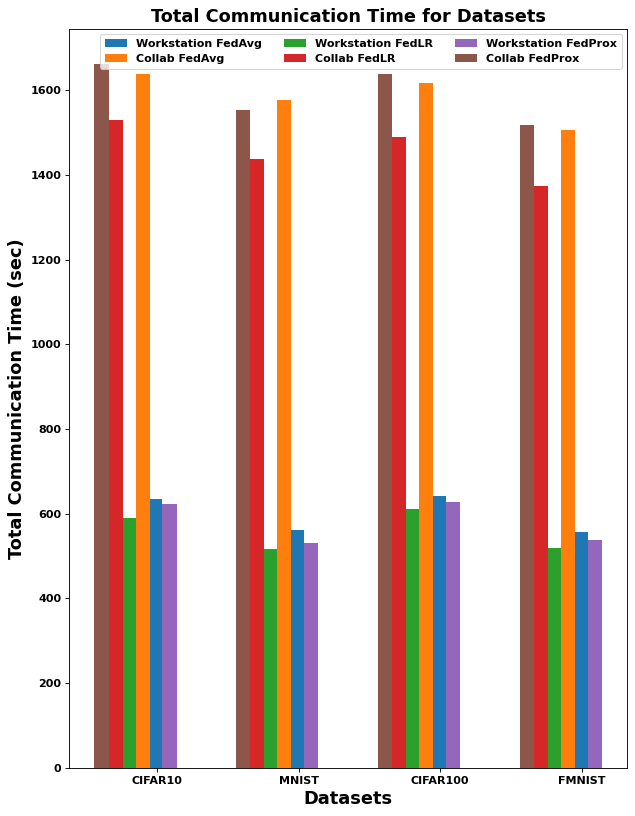
\includegraphics[scale=.36]{Images/Result Images/FinalGraphwithFedprox }
	\caption{Total Communication Time for Datasets.}
	\label{Finalgraph}
\end{figure}


Fig \ref{FedAvgC10}, \ref{FedLRC10}, and \ref{FedProxC10} all show similar accuracy and loss. This same pattern is seen in other datasets as well \cite{lecun1998mnist}  \cite{xiao2017fashionmnistnovelimagedataset} \cite{Krizhevsky09learningmultiple}. The detailed results can be found in table \ref{totaltimetable} and the visual representation in fig. \ref{Finalgraph}. In all the workstation results FedLR has shown the best results and FedProx is the second best. But in collab results it was mixed bag. As collab gives you a random T4 GPU in each instance which means the heterogeneity is more severe. Which lead to FedAvg performing better than FedProx in some cases.

% Please add the following required packages to your document preamble:
% \usepackage{multirow}
% \usepackage{graphicx}
\begin{table}[ht]
	\centering
	\caption{Total Communication Time with Different Datasets }
	\resizebox{\columnwidth}{!}{%
		\begin{tabular}{|l|l|l|l|l|}
			\hline
			Datasets                  & System      & FedLR (sec) & FedAvg (sec) & FedProx (sec) \\ \hline
			\multirow{2}{*}{CIFAR10}  & Workstation & 589.74      & 635.65       & 622.28        \\ \cline{2-5} 
			& Collab      & 1528.82     & 1638.73      & 1662.25       \\ \hline
			\multirow{2}{*}{MNIST}    & Workstation & 515.81      & 562.51       & 531.81        \\ \cline{2-5} 
			& Collab      & 1438.09     & 1576.74      & 1553.16       \\ \hline
			\multirow{2}{*}{CIFAR100} & Workstation & 611.08      & 641.14       & 628.44        \\ \cline{2-5} 
			& Collab      & 1490.00     & 1617.62      & 1637.13       \\ \hline
			\multirow{2}{*}{FMNIST}   & Workstation & 519.84      & 557.56       & 537.23        \\ \cline{2-5} 
			& Collab      & 1374.31     & 1504.77      & 1516.53       \\ \hline
		\end{tabular}%
	}\label{totaltimetable}
\end{table}
To interpret the results more easily Percentage difference has been calculated. Compariosn between FedLR and FedAvg as well as FedLR and FedProx. Table \ref{percentage_table} shows the detailed results. In workstation setting the proposed methodology has peformed better than FedAvg and FedProx. But as we have explained earlier in the case of Google Collab the results were a bit different. All test have been run several times and the full results are available at ``https://github.com/vipulhld001/flower".

% Please add the following required packages to your document preamble:
% \usepackage{graphicx}
\begin{table}[ht]
	\centering
	\caption{Percentage Difference of Communication Time with Different Datasets }
	\resizebox{\columnwidth}{!}{%
		\begin{tabular}{|l|l|l|l|l|}
			\hline
			Datasets & \begin{tabular}[c]{@{}l@{}}Workstation\\ FedAvg\end{tabular} & \begin{tabular}[c]{@{}l@{}}Collab\\ FedAvg\end{tabular} & \begin{tabular}[c]{@{}l@{}}Workstation\\ FedProx\end{tabular} & \begin{tabular}[c]{@{}l@{}}Collab\\ FedProx\end{tabular} \\ \hline
			CIFAR10  & 7.5\%                                                         & 6.9\%                                                    & 5.3\%                                                          & 8.3\%                                                     \\ \hline
			MNIST    & 8.7\%                                                         & 9.2\%                                                    & 3\%                                                            & 7.7\%                                                     \\ \hline
			CIFAR100 & 4.8\%                                                         & 8.2\%                                                    & 2.8\%                                                          & 9.4\%                                                     \\ \hline
			FMNIST   & 7.0\%                                                           & 9.0\%                                                    & 3.3\%                                                          & 9.8\%                                                     \\ \hline
		\end{tabular}%
	}\label{percentage_table}
\end{table}



\section{Conclusion}
The proposed algorithm has reduced the total communication time by a significant margin and has maintained fairness in the system while maintaining the accuracy of the models. The proposed algorithm has also been tested on two different devices to prove the improvements in communication rounds for a federated learning system with many slacker devices. Both FedAvg and FedProx are compared with the proposed work and proposed work has significantly improved over both of them. Using proposed methodology in IoT and Edge devices will make the Federated Learning process more efficient and robust.
\bibliographystyle{unsrt}
\bibliography{Sample}


\end{document}


